\chapter{Project}
\section{Language choice}
As both team members are working in different fields of employment and are experienced in different programming languages, there wasn't an obvious choice as in what programming language we would implement this project. Also, as Java has already been used by the team in Geneva, Java was out of question. Different programming languages have been taken into consideration and in the end Python seemed like a rather suitable language due to the following reasons:

\begin{itemize}
	\item simple syntax and commonly known language features
	\item mature language and standard libraries
	\item python's syntax enables programs to be written in a compact and readable style
	\item native support for large integers (\textit{BigInts}) and bindings for the GMP\footnote{GMP is a free library for arbitrary precision arithmetic, operating on signed integers, rational numbers, and floating-point numbers, see \url{https://gmplib.org/}.} library
	\item supports a lot of platforms
	\item many popular web development frameworks are implementated in Python
\end{itemize}

Throughout the project not all of the reason above turned out to be true or ideal. The drawbacks that we have experienced during the implementation of this project will be discussed at the end of this document.

\section{Project method}
The first step was to get a basic understanding of the CHVote protocol by reading the specification document and refreshing our knowledge about the cryptographic primitives used in the protocol. We decided to follow the "learning by doing" approach: while implementing an algorithm, we tried to understand how it works and how it interacts with other algorithms.

Before starting with the implementation, we created a timetable in order to track the project's progress. The idea of the timetable was to keep track of each individual algorithm and its implementation status, as well as appropriate unit tests and the review status of each algorithm. We made sure that all algorithms were reviewed by a different person than the one who implemented it. This way we were able to eliminate a lot of careless mistakes.

The following table is an excerpt from the timetable that we used, displaying the first algorithms that we implemented in an early stage of the project.

% TODO insert timetable
%\noindent
%\makebox[\textwidth]{
%	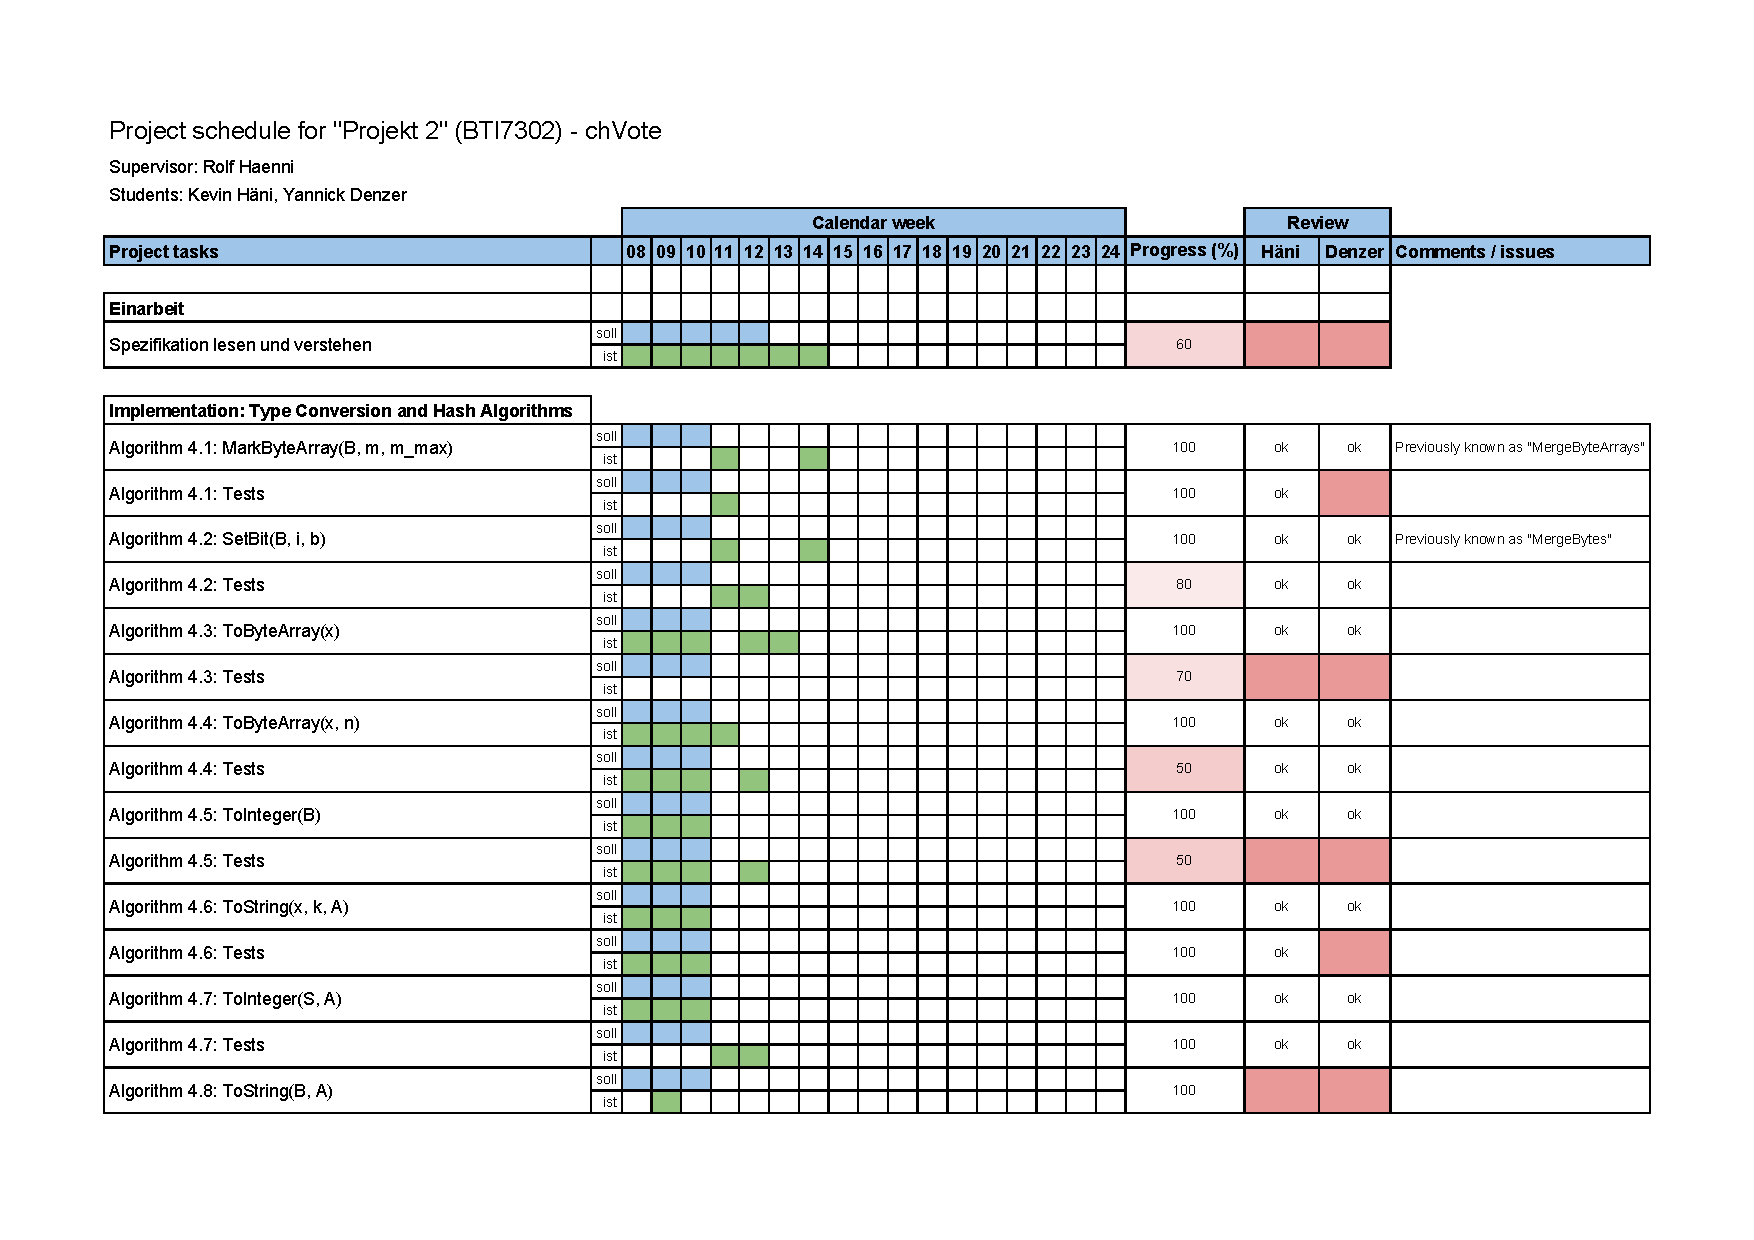
\includegraphics[width=1.1\textwidth]{images/timetable.pdf}
%}
